\section{剖面成像}
\label{sec:5.7}

野外剖面由一个炮点和沿测线分布的许多接收器得出的地震记录所组成\footnote{
此处的profile
(剖面)一词系专指共炮点排列而言,它与section一词是有区别的。后者专指时间剖面
(time section)。---译者
}。一个共炮点
道集剖面的偏移或者许多个相距颇远的共炮点道集剖面的偏移,需要建立与本书迄今所讨论
之任何概念、即爆炸反射面与观测排列延拓等概念是完全不同的概念基础,这样一种概念基
础是存在的,它的出现时间先于爆炸反射面或观测排列延拓(Claerbout,1970),而且看来比
这些概念还更具有基本意义。我把这老式的成像概念称作成像概念。

观测排列延拓概念看来得要求完全复盖炮点检波点空间,爆炸反射面概念则需要有许多
相距很近的炮点。另一方面,采用成像概念的剖面成像对沿炮点坐标轴的分布密度则没有
什么要求。只能用老式概念加以处理的数据组的例子就是声纳浮标,声纳浮标是一种带有无线
电传输装置的水听器,把它投掷船外,随着装备有空气枪的勘探船不断驶远,重复起爆激发
直至距该水听器的距离过大为止。根据互换原理可以宣称,如此所得数据等价于在一非常长
的检波点测线上采用单炮激发所得结果。

尽管技术进步使得沿检波点坐标轴能够有更大的采样密度,我们未必就愿意增大炮点空
间内的密度天只有廿四小时,而每两炮之间我们必须等待十秒钟才能使回声反射衰减
完。所以,给定了一定的勘探面积和一定的工作月数,我们就得以某种不可再削减的炮点密
度来完成任务。实际上,采用三维观测我们还愿意空间采样密度要小一点,炮点空间中的采样
密度不足对于剖面方法来说不过是个小小障碍。

同爆炸反射面方法与观测排列延拓法不一样,U/D概念很容易同多次反射的模拟与分析
结合起来。实际上,在《地球物理数据处理基础》一书中可以找到能够同时实现偏移和去交
混回响的巧妙算法,它原则上可以应用于野外剖面或倾斜叠加。

各种波动方程方法已经隐含暗示了进行风化层校正的一些新途径,迄今尚没有一种途径
能广泛为生产实践所接受,它出现得过早,没告诉人们将起较好作用的究竟是双平方根方程
DSR办法还是剖面成像办法。

所有这些考虑都说明值得再回顾一下剖面偏移法和成像概念,我们可能很容易就见
的这些概念或者以这种形式、或者以那种形式重新复兴起来。

\subsection{U/D成像概念}
\label{sec:5.7.1}

U/D成像概念宣称:反射面存在于地层内下行波波至时间与某一上行波波至时间相符一
致之处,图\ref{fig:mltp/udimage}以图形方式解释了这个概念。

观测排列延拓概念很容易同成像概念相混,因为用于描述它们的语句很相似:“炮
点向下延拓”听起来就像是“下行波向下延拓”
。头一个概念是指只涉及上行波场$U(s,g,z,t)$
的计算,第二个概念是指既涉及上行波$U(x,z,t)$又涉及下行波$D(x,z,t)$的计算。
U/D成像概念不包含特定的震源位置S;源可能就是下行平面波。

在剖面偏移法\footnote{
即共炮点道集的偏移。---译者
}中,在理论上下行波通常典型地是作为脉冲处理的,其旅行时间系由解
析方法求出或者用射线追踪方法求出。但是,采用前几章所述Fourier变换或有限差分方
法,可以按处理上行波的同样方式来处理下行波,这一点并无关紧要。上行波可以用直角坐
标系统表示,或者用下面要述及的时差坐标系统描述。

上行波与下行波的时间相符一致可以用若干方式定量描述,最直接的方式看来就是着
眼于两种波的互相关函数之零延迟时间,在$(x,z)$空间内处处显示出零值延迟时的互相关函数,就可形成映像。

上行波在时间上与一个下行波的最早波至符合一致就是证明存在有一反射面,不过,从
原理上说,还可以从这两种波了解到更多信息,上行波对下行波的振幅比就给出了反射系数
的信息。

在Fourier变换域内,乘积$U(\omega,x,z)\bar{D}(\omega,x,z)$
代表该互相关函数零延迟时的
值,反射系数比值则由$U(\omega,x,z)/D(\omega,x,z)$给出。这种比值存在许多困难,不但
分母可能为零,而且它在复平面异常区内可能有零点,这种事情发生在下行波虽遵守因果律但
不是极小相位的时候(见《地球物理数据处理基础》一书4.6节)。复共轭复数之相位等于
该复数倒数之相位,因而比值U/D与乘积$U\bar{D}$二者均具有相同之相位,看来你可以创造其他
的函数形式,使对U/D的理论要求可用U万的稳定性条件来折衷代替。

DonC.Riley( 1974
)曾提出过另一种形式的成像原理,即,在下行波初至之前
的所有时刻上行波必须为零,这种Riley形式
的原理曾在波动方程去混晌方法中得到应用。

\begin{figure}[H]
\centering
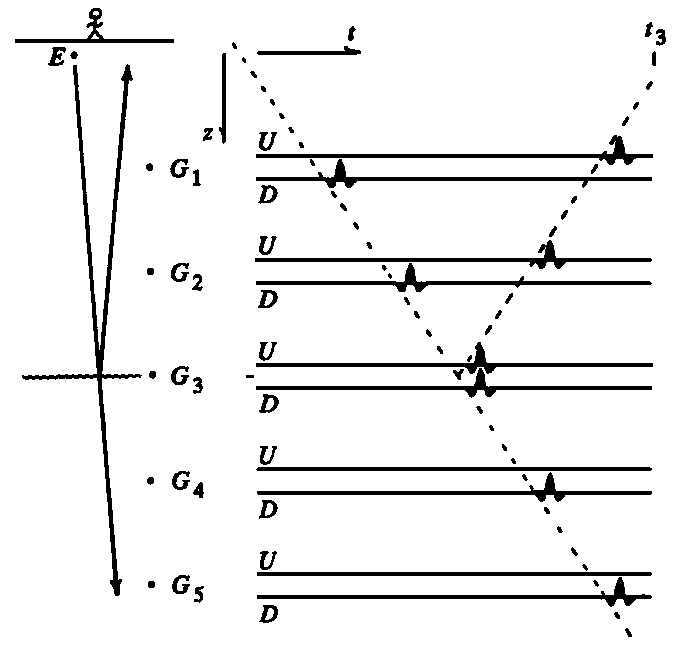
\includegraphics[width=0.65\textwidth]{mltp/udimage}
\caption[udimage]{以埋置检波器观测到的上行波与下行波。
扰动在时刻$t=0$离开地面,然后在相继渐次增大的各时刻通过
埋置地下的各接收器$G_1,G_2,...,G_5$而被观测到。在反射
面深度$Z_s$上,接收器$G_8$既记录到上行波也记录到下行波,
二者时间相符一致。较浅些的各接收器亦记录到这两种波,较深
的接收器则只记录到D。反射面映像基本原理阐明反射面存在于U
与D为时间相符一致之处(据Riley)。
}
\label{fig:mltp/udimage}
\end{figure}


\subsection{时差校正坐标系统内的偏移}
\label{sec:5.7.2}

如果地层在所有三维方向真是非均匀的,
我们可能很难指望一条地震测线的资料还完全
能有什么意义。可是反射地震学通常看来是起
作用的,即使只限于一条测线也是如此,这就
表明地层的层状模型是一种合理的出发起点。

因而,正常时差校正通常就是一个良好的起始
过程,从数学上说,正常时差校正是对付速度
随深度而变动的一种出色工具,但是在存在陡
倾角或广角谱(wide dip spectrum)情形下,其用途将大打折扣。

我早期的偏移程序曾经都是建立在由单个
剖面导出的概念基础上,将数据和波动方程变
换至某种时差校正坐标系统。这种实现偏移的
办法很适合于沿检波点坐标轴稀疏采样的资
料,当记录道所在地面的倾角变陡时,这时时
差校正就提供不了多大好处了。实际上,它倒
引进了不受欢迎的复杂性。无论有什么优点或
缺点,正常时差校正因其在工业生产领域内近
乎普遍通用而使我们不得不注意。

\subsection{检波点空间内的径向坐标与时差}
\label{sec:5.7.3}

我们的理论分析将放弃检波点坐标轴g而赞同采用以Snell参量p表示其特征的径向式坐
标轴(radial-like axis)。(这实际就是说与所应用的数据处理本身没关系,因为最后的
方程变换返回至炮检距空间简单得很)。现在定义的坐标系统将称作延迟的时差校正Snell
记录道坐标系统,在零倾角地层情形下,这种坐标系统内的理想数据在被向下延拓时是不改
变的,因而微分方程必须完成的工作量与数据偏离理想情形的程度成比例。与此类似,对数
据的空间采样的需要程度也随数据偏离理想情形的程度而成比例地増加,这种坐标系统采用
的各符号定义如下:
p---Snell射线参量$(\sin\theta)/v$;\\
$t_p$---由地面开始沿参量为々之射线传播的任何单程时间;\\
g---炮点距检波点的地面间距; \\
t'---地面至反射面沿射线的单程时间;\\
$\tau$---迆下埋置检波器的旅行时间深度,沿射线之单程时间;\\
t---地下埋置检波器所记录之旅行时间;\\
$v(p,t_p)$---新坐标内之分层速度函数$v'(z)$。\\
坐标系统建立在下列简单陈述的基础上:
(1)炮点至检波点之旅行时间为炮点至反射面的旅行时间之二倍再减去检波器之时间深
度;(2)射线传播所经水平距离等于对$v\sin\theta=pv^2$
的时间积分;(3)射线传播所经垂直距
离按计算水平距离的相同方式计算,但以余弦代替正弦
\begin{equation}
t(t',p,\tau)=2t'-\tau
\label{eq:ex5.7.1}
\end{equation}
\begin{equation}
g(t',p,\tau)=2p\int_0^tv(p,t_p)^2dt_p-p\int_o^{\tau}v(p,t_p)^2dt_p
\label{eq:ex5.7.2}
\end{equation}
\begin{equation}
z(t',p,\tau)=\int_0^\tau v(p,t_p)\sqrt{1-p^2v^2}dt_p
\label{eq:ex5.7.3}
\end{equation}
具有恒定t'值的面属于反射,具有恒定p值的面属于射线,具有恒定$\tau$值的面是基准面。可
惜,不可能以显式形式反演上述坐标系统使$(t',p,\tau)$成为$(t,g,z)$的一个函数,然
而,利用微分关系以解析方式进行反演是有可能的,根据Jacobi矩阵关系,应有
\begin{equation}
\begin{pmatrix}
\partial_t' \\
\partial_p \\
\partial_\tau
\end{pmatrix}=
\begin{pmatrix}
t_t' & g_t' & z_t'\\
t_p  & g_p  & z_p \\
t_\tau & g_\tau & z_\tau 
\end{pmatrix}
\begin{pmatrix}
\partial_t \\
\partial_g \\
\partial_z
\end{pmatrix}
\label{eq:ex5.7.4}
\end{equation}
仅只在它们能导致显著简化的场合才进行微分时,就可得出,Fourier变量的变换方程
\begin{equation}
\begin{pmatrix}
-\omega ' \\
k_p \\
k_\tau
\end{pmatrix}=
\begin{pmatrix}
2 & g_t' & 0\\
0 & g_p  & z_p \\
-1 & g_\tau & z_\tau 
\end{pmatrix}
\begin{pmatrix}
-\omega \\
\partial_g \\
\partial_z
\end{pmatrix}
\label{eq:ex5.7.5}
\end{equation}

应注意,式\ref{eq:ex5.7.5}是涉及Fourier变量的一个线性变换,但是系数却包含原有的时间
变量和空间变量。因此,式\ref{eq:ex5.7.5}同时处于两种变量域内,只要假设二阶导数可忽略坐
标框架本身的导数,这种关系式就能有效成立,这经常是一项宽容的假设,相当于有几分像
球形扩散校正。

要是我们继续在这里讨论非零炮检距情形,我们可能要陷入繁琐细节的泥潭而不能自拔
了。现在使问题具体化到零炮检距情形,即令$p=0$,于是得
\begin{equation}
\begin{pmatrix}
-\omega ' \\
k_p \\
k_\tau
\end{pmatrix}=
\begin{pmatrix}
2 & 0 & 0\\
0 & 2t'-\tau  & 0 \\
-1 & 0 & v 
\end{pmatrix}
\begin{pmatrix}
-\omega \\
\partial_g \\
\partial_z
\end{pmatrix}
\label{eq:ex5.7.6}
\end{equation}
不妨将式\ref{eq:ex5.7.6}代入向下延拓检波器时所采用的单平方稂方裎内,从而M读方裎变换成
新坐标系统内的一项延迟方程。

\subsection{关于神奇奥妙之比例因子的历史注释}
\label{sec:5.7.4}

我首次用波动方程对反射烛震资料作的偏移曾是以概念为基础,头一个波动方程偏
移程序是频率域程序而且是用合成剖面作出来的。由于人们一般都忽视这样的成果,我決心
完成一项野外数据的实际试验。频率域方法曾被讥为是“学究气”的,我却发现了我能够用
Z变换分析中的双线变换把15°波动方程转换至时间域。就实践问题而论,共炮点道集偏移程
序显然是可以应用于时间剖面的,不过理论证明却并非易事,在那个时斯我曾把爆炸反射面
概念看作是荒谬的类比,尚未把它当成是导出偏移程序的基础。

以有限差分对第一个零炮检距剖面进行偏移时所曾采用的实际处理办法比后来由
Sherwood ( Loewenthal等,1976
)所介绍且为一般所采用的处理办法要迂迴复杂得多。
时差校正坐标系统内的共炮点道集偏移方程(equation for profile migration )有许多
项,略去所有以炮检距作为系数的那些项(因为你正在试图偏移的是某种零炮检距剖面),
给你留下的一个方程将类似于延迟的15°外推方程,但存在有一个差别,即项有奇妙的
比例系数$[t'/(2t'-\tau)]^2$,这就是我曾采用过的方程。随着旅行时间深度$\tau$从零増大至终
止深度$t'$,该奇妙的系数缓慢地从1/4増大到1。

可惜我的导出过程太复杂,以致几乎没什么人能领会它(你要注意,我并没有完全将它
包括在这里)。我在1972年发表的论文包括有该导出结果,不过采取的介绍方式能使你通晓
概念上比较简单的情形、即地震剖面由下行平面波震源所形成。这种较简单的情形能使你迅
速得出偏移方程,但是奇妙的系数不在了,按深度平均之后,该系数平均值为二分之一
。有一天,Sherwood曾打电话给我,挑战式地问我为什么该系数不用它的平均值1/2来代替,
我提不出什么实际理由,今天我也不能回答为什么。所以他放弃了我的褶积导出方法而选取
爆炸反射面模型作为假设,从而很容易地获得了所需要的值1/2
。以后当我和Doherty,
Muir及Clayton等的研究成果发展了观测排列延拓概念时,我对这个奇妙的系数就更感到心
安理得了。

我的第一本书《地球物理数据处理基础》描述了U/D概念如何可以用于处理偏移、速度
分析及多次波压制这三种问题,在这三类应用中,仅有零炮检距剖面偏移这一类使波动方程
的一套方法成了常规实际处理的一部分,U/D成像概念迄今依然普遍被遗忘而被Sherwood
的爆炸反射面概念所代替。


